\documentclass{scrartcl}
\usepackage{german}
\usepackage[utf8]{inputenc}
\usepackage[german]{babel}
\usepackage{amssymb}  % advanced mathematical symbold
\usepackage{graphicx} % using graphics
\usepackage{fancyhdr} % for the head of the page
\usepackage{lastpage} % makes page numbers work
\setlength{\parskip}{\medskipamount} % thats reasonable
\setlength{\parindent}{0pt}

\usepackage{wrapfig}


%%%%%%%%%%%%%%%%%%%%%%%%
% Kopf- und Fusszeilen %
%%%%%%%%%%%%%%%%%%%%%%%%
\pagestyle{fancy}
\lhead{
    \begin{tabular}{ll}
        Felix Karg & 4342014\\
    \end{tabular}
}
\chead{Superturingmaschinen}
\rhead{
    \begin{tabular}{rr}
        \today{} \\
        Seite \thepage{} von \pageref{LastPage}
    \end{tabular}
}
\lfoot{}
\cfoot{}
\rfoot{}

\title{Superturingmaschinen}
\author{Felix Karg}

%%%%%%%%%%%%%%%%%%%%%%%%
% Anfang des Dokuments %
%%%%%%%%%%%%%%%%%%%%%%%%
\begin{document}
\maketitle

\textbf{\large {Abstract:} } \\
Superturingmaschinen sind eigentlich nur Turingmaschinen, die wir nach dem Ende
der Zeit betrachten können, wodurch wir also z.B. das klassische Halteproblem
lösen. Turingmaschinen sind ein klassisches Beispiel für Hypercomputation, also
eine Berechenbarkeitsstufe über traditionellen Turingmaschinen, die allerdings
Physisch fragwürdig realistisch umzusetzen ist. Dennoch ergeben sich ein paar
interessante Eigenschaften, die genauer beleuchtet werden sollen.


\section{Berechenbarkeit}
Es gibt (wie allgemein bekannt ist) verschiedene Stufen der Berechenbarkeit,
wobei die einfachste kombinatorische Logik (einfache, nicht-Zyklische
Schaltkreise) ist, und weitergehende über $DEA$ (Determistische Endliche
Automaten), $PDA$ (Push-Down-Automaton, dt: Kellerautomaten)
bis hin zu Turingmaschinen, die schon bereits alles Berechenbare berechnen
können. Häufig wird also z.B. eine Programmiersprache daran gemessen, ob sie
Turingvollständig ist, ob also alle berechenbaren Funktionen berechnet werden
können. Neben Turingmaschinen gibt es (in den für realistische berechenbarkeit
betrachteten Bereichen) auch andere Modelle der Berechenbarkeit, z.B.
Registermaschinen, Generell-Rekursive Funktionen oder das Lambda-Kalkül.


\subsection{Konstrukt Turingmaschine}
Eine Turingmaschine ist eigentlich eine einfache, konzeptionell aber
robuste Konstruktion. Ich werde gleich noch näher darauf eingehen dass es
verschiedene, aber im Endeffekt äquivalente, Turingmaschinen gibt. (hier keine
formale Definition, da es nicht Hauptteil des Vortrages ist sowie wenig
hilfreich für das Verständnis). \\
Im Kern besteht eine Turingmaschine aus folgenden Elementen: Ein Band, das
ein Anfang hat aber nach rechts hin unendlich lange ist, also kein Ende hat.
Die eigentliche Maschine besteht aus einem kombinierten Lese- und Schreibkopf,
welcher auf dem Band operiert. Neben dem Initialzustand hat sie lediglich eine
endliche Menge an Zuständen. \\
Pro 'Berechnungsschritt' passiert nun folgendes: Die Turingmaschine liest ein
Zeichen vom Band und entscheidet in Abhängigkeit ihres momentanen Zustandes was
sie als nächstes tut. Möglich sind: Das aktuelle Zeichen so belassen, es
überschreiben, das Band nach rechts oder links bewegen, sowie entsprechend der
Übergangsfunktion meistens den Zustand wechseln.


\subsection{Eigenschafen von Turingmaschinen}
Relevant für uns ist im folgenden, dass es gewisse Definitionen beziehungsweise
Arten von Turingmaschinen gibt, die der vorgestellten Äquivalent sind. Ein
Beispiel wäre eine Turingmaschine die auf zwei oder mehreren Bändern rechnet
(die jeweils Unendlich lang sein können), eine die auf einem Band rechnet das
in beide Seiten unendlich lange ist, eine die in ihrem Alphabet nur $\{0, 1\}$
hat sowie eine die ein beliebig langes, endliches Alphabet zur verfügung hat
(Äquivalent in dem Sinne natürlich, dass wir jeweils nur eine lineare differenz
haben, bzw. eben dass nach $\omega$ Schritten kein unterschied festzustellen
ist.). Eine sehr interessante Eigenschaft ist, dass unsere Turingmaschine mit
ihren Endlich vielen Zuständen eindeutig definiert ist, Sie also auch
entsprechend Codiert werden kann und von einer anderen gelesen und Simuliert
werden kann. Daraus ergibt sich auch dass eine Turingmaschine gleichzeitig
mehrere simulieren kann. \\ Außerdem gibt es das Halteproblem, also dass
bereits bei einer Turingmaschine mit sehr wenigen Zuständen kein Zuverlässiger
Algorithmus existieren kann, der entscheidet ob diese irgendwann hält
(Terminiert, ein Ergebnis liefert) oder eben nicht. Das Halteproblem für
gewöhnliche Turingmaschinen ist für uns aber im folgenden nur von begrenztem
Interesse.


\subsection{Aussagentypen}
Eine Teilmenge $M \subseteq \mathbb{N}$ ist genau dann von einer Turingmaschine
aufzählbar (oder rekursiv aufzählbar) sofern es eine Turingmaschine gibt, die
in beliebiger Reinfolge alle Elemente dieser Menge auf das Band schreiben
kann. Eine solche Menge wird $\Sigma_1$-Menge genannt, wenn es eine
$\Sigma_1$-Aussage $\phi$ gibt, die über Logik (Arithmetik) erster Stufe
aufgebaut ist. Also der Form $\phi = \exists m_1...\exists m_k \heartsuit$,
bei der die Quantoren über die natürlichen Zahlen reichen dürfen sowie in
$\heartsuit$ keine weiteren ungebundenen Quantoren vorkommen dürfen und nur
eine freie Variable darin vorkommen darf, sodass $M = \{n \in \mathbb{N}\ |\
\phi(n)\}$. Dies entspricht nun genau der Klasse NP.

% Turingmaschinen, sowie Generell Rekursive Funktionen (Gödel) als auch das
% Lambda-Kalkül (Church) sind nun insofern gleichmächtig, als dass sie alle
% $\Sigma_1$-Aussagen, und die damit beschriebenen Mengen, ausdrücken können.


% Allgemein Rekursive Funktionen (Gödel), das Lambda-Kalkül (Church) sowie
% Turingmaschinen (Turing) werden häufig als Äuquivalent mächtige
% Berechenbarkeitsdefinitionen betrachtet. Das gilt erstmal nur für
% $\Sigma_1$-Aussagen, was Quantifizierungen über Variablen einschließt
% ($\exists e : ...$), also (bekannte) Existentielle Prädikatenlogik, oder
% Existenzielle Logik erster Stufe. An dieser stelle wird auch kurz darauf
% eingegangen was der Unterschied zu $\Sigma_1$-Aussagen ist, und warum
% das so ist. Interessanterweise unterscheiden sich die Berechenbarkeitsmodelle
% bei $\Sigma_1^1$-Aussagen, also inwieweit und welche von welcher Art als
% 'Berechenbar' gelten und welche nicht. Aufgrund eines interessanten Umstandes
% sind Superturingmaschinen dazu in der Lage, sowohl $\Sigma_1^1$-Aussagen als
% auch $\Pi^1_1$-Aussagen zu entscheiden (wozu Turingmaschinen eindeutig nicht in
% der Lage sind). Darauf wird hier weiter eingegangen.


\subsection{Limitierungen von Turingmaschinen}
Wenn wir allerdings alle ungebundenen $\exists$-Qantoren in unseren $\Sigma_1$-Aussagen mit
$\forall$-Quantoren ersetzen, dann werden diese zu $\Pi_1$-Aussagen, die unsere
Turingmaschine nun im Allgemeinen nicht mehr entscheiden kann, da sie durch
alle Natürlichen Zahlen iterieren müsste, was bekanntermaßen nicht Terminiert.
Das wäre nun genau die Klasse von Problemen in co-NP, die sich also in
Polynominieller Zeit widerlegen lassen.
% Außerdem gibt es das bereits angesprochene Halteproblem.


\newpage


\section{Unendlichkeit}
Umgangssprachlich verwendet man einfach das Wort 'Unendlich', und im Normalfall
ist auch allen beteiligten klar, worum es eigentlich geht. Damit es hier
genauso ist, und um ein wenig zwischen verschiedenen zu differenzieren benenne
ich im folgenden zwei verschiedene Arten der Unendlichkeit. Eine ist gemeint,
die andere explizit nicht. Ich beschreibe beide nun als jeweils neue Klassen
von Zahlen, die allerdings konzeptionell nichts Neues, sondern bereits
Altvertrautes sein sollten.


\subsection{Kardinalzahlen}
Kardinalzahlen sind Zahlen die Kardinalitäten angeben, also Beispielsweise die
Anzahl von Elementen in einer Menge ($|\{\square, \nabla, \heartsuit \} | =
3$). Soweit sind Kardinalzahlen also nicht von Natürlichen Zahlen zu
unterscheiden, aber wir sind ja auch noch bei endlichen Mengen. Sobald wir
unendliche Mengen betrachten, Beispielsweise $\mathbb{N}$, wird es interessant.
$|\mathbb{N}| = \aleph_0$, $\aleph$ ist nun ein Buchstabe aus dem Häbräischen
Alphabet. Wie bekannt sein sollte ist $\mathbb{N}$ abzählbar unendlich Groß,
genauso wie $\mathbb{Z}$ und $\mathbb{Q}$. Es ist also klar, dass $\aleph_0 +
\aleph_0 = \aleph_0$ ($\mathbb{Z}$), sowie $\aleph_0 * \aleph_0 = \aleph_0$
($\mathbb{Q} \cong \mathbb{Z} \times \mathbb{N}$). Dies ist eine Art der
Unendlichkeit auf die ich im folgenden nicht weiter eingehen werde, wer ein
Tieferes verständnis diesbezüglich möchte, ein schönes Gedankenexperiment dazu
ist Hilberts Hotel.
% Ich werde hier nicht weiter auf z.B. die reellen Zahlen
% eingehen, da nicht feststeht welche Kardinalzahl diese exakt Haben, bis auf
% dass diese größer ist als $\aleph_0$.


\begin{wrapfigure}{R}{0.5\textwidth}
    \centering
    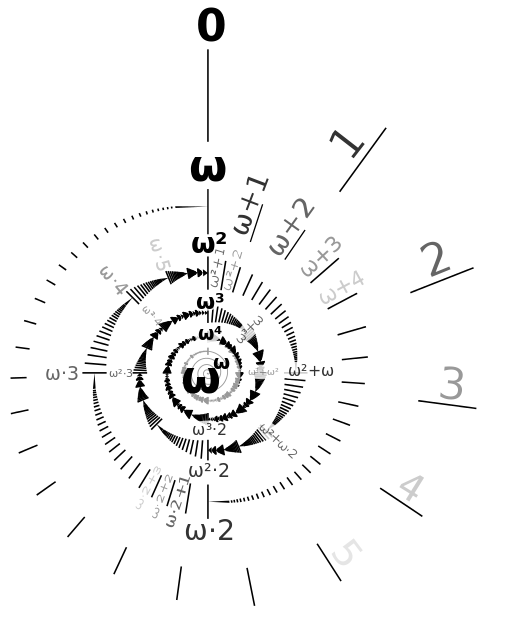
\includegraphics[width=5cm]{ordinal.png}
    \caption{\label{fig:ordinal.png}Ordinaler Zahlenstrahl}
\end{wrapfigure}


\subsection{Ordinalzahlen}
Eine andere Art von Unendlichkeit, mit der wir auch vertraut sind, beschreiben
die Ordinalzahlen.  Wir fordern eigentlich nur eine Eigenschaft: und zwar dass
die Ordnung erhalten bleibt. Anfänglich sind wir wieder äquivalent zu den
Natürlichen Zahlen, da diese bereits eine Wohlordnung haben. Wenn wir nun einen
Zahlenstrahl betrachten, Zeichnen wir einen solchen häufig mit $\infty$ am
rechten Ende, umgangssprachlich unendlich. Dieses Zeichen ist nicht Element der
Natürlichen, Reellen oder sonstigen Zahlen, sondern bezeichnet eher ein Element
größer als alle die wir aufschreiben oder uns vorstellen könnten. Wir
definieren uns nun ein Element $\omega$, das direkt rechts daneben anzuordnen
ist, also das erste Element außerhalb, oder rechts neben, eher nach, dem
Zahlenstrahl. Es sollte klar sein dass es strikt größer ist als alle
vorhergehenden Ordinalzahlen, also z.B. alle Zahlen die auch Natürliche Zahlen
wären. Die frage nach $\omega - 1$, also der Ordinalzahl vor $\omega$, kann
nicht beantwortet werden und macht auch wenig Sinn. Intuitiv: es ist nicht
möglich eine feste Zahl direkt vor 'unendlich' zu definieren, denn könnten wir
das, könnten wir diese Zahl so weit erhöhen (um 2) und wären größer als
$\omega$, die ja die größte Zahl gewesen sein soll. Allerdings ist zu beachten,
dass $1 + \omega = \omega \neq \omega + 1$. Intuitiv kann man wieder sagen dass
eben kein klar definiertes Element davor, wohl aber ein strikt größeres Element
danach gibt, oder dass man einen Zahlenstrahl wohl auch bei 2 anfangen kann,
dieser entsprechend immernoch gleich lang ist, aber wenn man ein Element nach
dem Zahlenstrahl hinzufügt, muss es immer erst nach dem Zahlenstrahl, strikt
hinter allen anderen Elementen davor, angeordnet sein. Genauso ist $\omega +
\omega = \omega * 2$, oder $\omega * \omega = \omega ^ 2$.


\section{Superturingmaschinen}
Superturingmaschinen klingen jetzt erstmal total super, und das sind sie auch.
Eigentlich sind es nur Turingmaschinen, außer dass ihre Schritte in
Ordinalzahlen gezählt werden, dass es also Schritte $\omega$, $\omega + 1$,
etc. quasi nach dem Ende der Zeit gibt, wo sie einfach weiterrechnen können.
Dadurch lösen wir das klassische Halteproblem von Turingmaschinen, da wir
einfach schauen können ob unsere Superturingmaschine (die sich ja sonst nicht
unterscheidet) nach dem Ende der Zeit bereits angehalten hat oder eben nicht.


\subsection{Verhalten bei Grenzen}
Was natürlich immer passieren kann, ist dass eine Superturingmaschine nicht
anhält, und ständig weiter eine Zelle mit 1 und anschließend mit 0 beschreibt.
In einem solchen fall (oder allgemein, wenn sie nicht hält) muss definiert
werden, was anschließend, in Schritt $\omega$ der folgende Zustand sein soll. Meta: An
diesem Punkt kann auf Supertasks hingewiesen werden, ein Beispiel wäre das
umschalten eines Lichtschalters nach immer halben Zeitintervall zuvor, also
angefangen bei 1s, 0.5s, 0.25s, ... wäre er in Sekunde 2 bei $\omega$
angelangt, allerdings ist bei ständigem umschalten eines Lichtschalters nicht
definiert, in welchem Zustand er anschließend, also nach sekunde 2, ist.
Außerdem gibt es auch keine eindeutige Antwort, da es gleichzusetzen wäre mit
'Ja, Unendlich ist gerade' oder eben dem Gegenteil davon. Allerdings sollte das
Publikum bereits mit Supertasks im allgemein vertraut sein. Da davon nicht
auszugehen ist, werde ich sie kurz erwähnen, aber dann weitermachen mit: eine
Turingmaschine die nicht Terminiert, in welchem Zustand ist sie zum Zeitpunkt
$\omega$? Weil: es kann einer von vielen sein, gleichzeitig eines von auf die
verschiedensten weisen beschriebenes Band. Und wieder: egal wie man's festlegt,
kann es gut passieren dass Eindeutig ist wie viele und welche Schritte bisher
notwendig gewesen sein müssen, also dass $\omega$ in einem solchen fall nicht
'nach' dem Zahlenstrahl kommt. Dementsprechend definiert man es folgendermaßen:
Sofern die Turingmaschine hält, ist sie auch nach beliebig vielen weiteren
schritten in ihrem Finalen zustand. Ist dies allerdings nicht passiert, wird
der Schreib-/Lesekopf wieder auf den Anfang gesetzt, sowie die
Superturingmaschine auf ihren Startzustand. Der einfachheit halber nehmen wir an dass
wir nur nuller (default) und einser auf unserem Band haben können. Eine null
wird nun an Schritt $\omega$ überall dort stehen wo entweder keine Eins
geschrieben wurde, oder nur endlich oft eine Eins geschrieben wurde. Eine Eins
steht hingegen überall dort, wo zu mehr als endlich vielen Zeitpunkten eine
Eins stand, bis hin zu von Anfang an (durchgehend). Dementsprechend ist der
Wert einer jeden Zelle entsprechend ihres Limeswertes (Grenzwertes), und die
Turingmaschine ist wieder auf Anfangszustand, allerdings mit möglicherweise
verändertem Band.


\subsection{Fähigkeiten}
Superturingmaschinen können nun Natürlich zum einen alles tun was normale
Turingmaschinen auch können. Außerdem können sie, wie wir eben gesehen haben,
entscheiden ob eine normale Turingmaschine hält oder nicht. Genauso können sie
natürlich neben dem Simulieren von normalen Turingmaschinen auch
Superturingmaschinen simulieren. Was sie allerdings auch entscheiden können
sind $\Sigma_1^1$-Aussagen, also Aussagen der Form 'Es gibt eine Funktion
$\mathbb{N} \rightarrow \mathbb{N}$ so dass ...', sowie $\Pi^1_1$-Aussagen,
also Aussagen der Form 'Für jede Funktion $\mathbb{N} \rightarrow \mathbb{N}$
gilt ...'. Was Superturingmaschinen immernoch nicht können, ist Beliebige
0/1-Folgen auf das Band schreiben. Auch eine Superturingmaschine hat nur
endlich viele Zustände, und damit gibt es Aussagen die nicht Abgebildet
werden können, ein einfaches Beispiel wären $\Sigma_1^2$-Aussagen. Was
wir uns allerdings auch klarmachen können, ist dass sie Selbstverständlich
alle $\Sigma^0_n$-Aussagen = $\Sigma_n$-Aussagen sowie $\Pi_n$-Aussagen
entscheiden können. Was allerdings immernoch nicht der Fall ist, dass es für
jede beliebige 0/1-Folge eine Superturingmaschine gibt, die diese letztendlich
auf das Band schreiben kann. Das Lost-Melody-Phänomen (wozu wir später evtl
kommen) besagt allerdings dass manche dieser 0/1-Folgen dennoch erkannt werden
können.


\subsection{Überlegung}
Wann hält folgende Superturingmaschine: Im initialzustand, halte, wenn eine
Eins zu lesen ist, andernfalls schreibe eine 1, schreibe wieder auf dasselbe
Feld eine 0 und gehe nun einfach nur nach rechts. Diese Superturingmaschine
hält nun erstmal (offensichtlich) nicht, auch nach schritt $\omega$ und erstmal
jedem weiteren Grenzzustand wird an der Initialen zelle die Null stehen.
Allerdings, nach schritt $\omega^2$ ändert sich das, da nun die Eins mehr als
nur endlich oft in dieser Zelle zu sehen war. Dementsprechend hält die
Superturingmaschine.


\subsection{Halteverhalten von STM}
Die frage ist nun natürlich wie lange genau eine Superturingmaschine braucht,
um zu halten. Eine Ordinalzahl $\alpha$ ist Stempelbar, wenn es eine
Superturingmaschine gibt, deren Programm bei Input 0 genau in Schritt $\alpha$
hält. Eindeutig sind auch
alle Natürlichen Zahlen $n$ Stempelbar, einfach durch eine Turingmaschine die
nach $n$ Zuständen hält. Limeszustände einfach durch wechseln der Zelle, bis
sie vom Initialzustand eine eins enthält bei der man dann halten kann.
Auch sind also eindeutig $\alpha + 1$ bis $\alpha + \omega$ Stempelbar, und
insgesamt alle Zahlen von $0$ bis $\omega^2$, und weiter, insofern $\alpha$
Stempelbar ist, ist es auch $\alpha + \beta$ mit $\beta \leq \omega^2$.
Nun scheint es erstmal so, als ob jede Ordinalzahl Stempelbar ist. Dem kann
allerdings nicht der Fall sein, da es überabzählbar unendlich viele
Ordinalzahlen gibt, und gerade mal abzählbar unendlich viele Turingmaschinen /
Programme / Zustandskombinationen. Die erste Lücke finden wir also
folgendermaßen: wir simulieren alle möglichen Turingmaschinen mit input Null,
und zwar so, dass diese auch jeweils $\omega$ Zeitschritte machen während wir
es auch tun. Bei unserem $\beta$ an dem nun keine Turingmaschine hält, brauchen
wir nun eben noch genau $\omega$ viele Zeitschritte um dies zu erkennen, und
können also entsprechend an $\beta + \omega$ halten, was also $\beta + \omega$
Stempelbar macht. Damit ist die Lücke mindestens $\omega$ groß. außerdem gibt
es nun für jede Stempelbare Ordinalzahl eine Lücke die mindestens so groß ist,
und es gibt mindens $\alpha$ davon. je nachdem wie viel Zeit verbleibt liefere
ich im Vortrag auch jeweils den Beweis dazu (Theorem 3.5 und 3.6).



% Meta: Im Paper ist nun abhängig von der Annahme, es gibt nicht-Stempelbare
% Ordinalzahlen ein Beweis für die erste Lücke, die $\omega$ groß ist. Die
% Frage ist nun, ob folgender Beweis genau das gegenteil beweist: \\
% Angenommen, es gibt eine nicht-Stempelbare Limes-Ordinalzahl $\beta$, und
% aufgrund des Speedup-Lemmas sind daher auch $\beta + \omega$ nicht Stempelbar.
% Allerdings muss es ein Programm geben, das davor gehalten hat, also $\alpha <
% \beta$. Wir können nun annehmen dass $\alpha$ der vorherige Limesordinal ist,
% andernfalls können wir auch ein Entsprechendes Programm Konstruieren (Beweis im
% Paper). Wir modifizieren nun das Programm das urpsrünglich an $\alpha$ hält
% folgendermaßen, um an $\beta$ zu halten: Zuerst fügen wir einen zusätzlichen
% Initialzustand hinzu, der Terminiert sollte er eine Eins lesen und ansonsten
% eins nach rechts geht (sollte es situationen geben in der wieder quasi zum
% Anfang des Bandes zurückgegangen wird, fügen wir als darauffolgenden Zustand
% auch einen ein der einfach nur eins nach rechts geht). Und wir verändern die
% momentane halt-bedingung so, dass wir stattdessen eine eins in genau die erste
% Zelle auf dem Band schreiben, und fortan nur rachts gehen. Im nächsten
% Ordinal-Limeszustand werden wir nun Terminieren, und dieser muss nun $\beta$
% sein. Dementsprechend gibt es keine Lücken in den Ordinalzahlen, also es gibt
% für mindestens jeden Limesordinalzustand eine Turingmaschine die an genau
% diesem Hält.




% Bei gewöhnlichen Turingmaschinen gilt: Die Anzahl der schritte, die eine
% Turingmaschine machen kann um bis dahin sicher angehalten zu haben oder nicht
% mehr zu Terminieren, ist abhängig von der Anzahl der Zustände, wobei diese
% Funktion (die für die Anzahl der Zustände die Maximale Schrittzahl zurückgibt)
% nicht Berechenbar ist, und vermutlich einer der am Stärksten wachsenden
% bekannten Funktionen ist. Meta: das nicht-berechenbar für Turingmaschinen
% würde ich möglicherweise an diesem Punkt ein wenig weiter ausführen, alternativ
% (je nach dem wie viel Zeit bereits verstrichen ist) werde ich es komplett
% weg lassen. Eine durchaus interessante Eigenschaft von Turingmaschinen ist
% folgende: Jede Berechnung hält entweder nach abzählbar vielen schritten oder
% verfängt sich in einem wiederholendem Zyklus, aus dem Sie nicht ausbrechen
% werden kann. \\
% Der Beweis dafür ist in einem der Paper, allerdings werde ich ihn weder hier
% noch im Vortrag wiedergeben (solange niemand danach Fragt), da es zwar durchaus
% ein Interessanter Fakt ist, allerdings der Beweis für das Verständnis (vor
% allem im Folgenden) im gegensatz zum eigentlichen Fakt nicht relevant ist. \\
% Terminologie: eine Ordinalzahl, an der eine Superturingmaschine halten kann,
% wollen wir im folgenden Stempelbar nennen.
% Daraus ergibt sich außerdem folgendes: Falls $\alpha + n$ Stempelbar ist,
% so ist dies auch $\alpha$. $n$ ist hier natürlich eine Natürliche Zahl,
% und alles was dies sagt ist wir können eine Turingmaschine natürlich auch
% bei jedem nicht-Grenzzustand frühzeitig beenden, sofern wir nur endlich viele
% Schritte im folgenden nicht machen. Meta: Ja es geht jetzt und auch im
% folgenden um die Stempelbarkeit, nicht direkt die Berechenbarkeit.
% Genauso funktioniert dies auch andersrum, wenn wir nach $\alpha$ Schritten
% halten sollten, können wir natürlich auch noch endlich viele ($n$) anschließen,
% und kommen also bis hin zu $\alpha + n$. \\
% Was klar sein sollte ist dass es viel mehr Ordinalzahlen gibt als Stempelbar
% sind, da wir jede Turingmaschine als Natürliche Zahl kodieren können (endlich
% viele Zustände!) gibt es selbst für abzählbar unendlich viel möglichen Input
% nur abzählbar unendlich viele haltende Stiuationen. Da Es aber strikt mehr
% Ordinalzahlen gibt, muss es einige Ordinalzahlen geben die nicht Stempelbar
% sind. Ein Theorem besagt nun dass es Große Lücken innerhalb der Ordinalzahlen
% gibt, die nicht Stempelbar sind. Ein anderes, dass es viele Solcher Lücken gibt,
% und wieder ein anderes dass es Große Blöcke von nicht-Stempelbaren Zahlen gibt.
% Die idee ist, dass man jetzt kurz darüber nachdenkt. \\


\section{Unendliche Halteprobleme}
Falls noch Zeit sein sollte und alles vorhergehende wirklich verstanden wurde,
gibt es möglicherweise noch ein kleineres Kapitel über Halteprobleme nach dem
Ende der Zeit, da wir zwar bereits das klassische Halteproblem 'gelöst' haben,
allerdings gibt es auch etwas Analoges für Superturingmaschinen. Hier sind
nicht $H = \{(p, x)\ |\ p$ hält bei input $x\}$ und $h = \{p\ |\ p$ hält bei
input $0 \}$ gleich, wie dies bei gewöhnlichen Turingmaschinen der fall ist,
und warum das so ist.



\section{Meta}
Hier noch ein wenig mehr META: Bezüglich der Aussagentypen werde ich das ganze
wohl auf den Folien dann ein wenig ausführlicher und hoffentlich viel
verständlicher machen. Natürlich ist angedacht dass aufkommende Fragen immer
sofort zu stellen sind und dementsprechend beantwortet werden. Möglicherweise
wird es noch ein paar kleinere änderungen geben, eventuell bekomme ich sogar
einen kurzen Teil über Effektive Topoi unter, allerdings dann dazu dort mehr.
Auch: Ich hoffe das bereits erwähnte Lost-Melody-Theorem unterzubekommen, das
einfach gesagt besagt dass es 0/1-Folgen (Sprachen) gibt die zwar erkannt
werden können, die aber keine Superturingmaschine schreiben kann, was mit den
Unendlichen Halteproblemen zu tun hat.


\end{document}
